% !TeX spellcheck = en_GB
A standard approach to modeling open quantum systems is the collision model.
The system under consideration interacts with a series of ancilla systems through a unitary transformation on the combined system-ancilla state \cite{Lorenzo_2017}. After a short interaction time $\Delta t$, the ancilla systems are traced out to receive the system state.
This type of interaction will in general lead to entanglement between system and ancilla.
To ensure the ancilla and system states remain pure, we follow the approach used in \cite{beyer2020}:
let $\rho_S$ be the density operator of the system under consideration and $\ket{\psi_A}$ the state of the ancilla system.
Given $\Delta t \ll 1$ the time evolution of $\rho_S$ under $H_{AS}$ acting on the combined system is
\begin{align}\label{coll_eq}
\rho'_S & = \mathrm{Tr}_A \{ e^{-i H_{AS} \Delta t} (\ket{\psi_A} \bra{\psi_A} \otimes \rho_S) e^{i H_{AS} \Delta t} \} & = \rho_S - i \Delta t [\expval{H_{AS}}{\psi_A}, \rho_S] + O(\Delta t^2).
\end{align}

In the continuous limit equation \ref{coll_eq} leads to von-Neumann dynamics on the system:

\begin{align*}
	\dot{\rho}_S = - i [\expval{H_{AS}}{\psi_A}, \rho_S].
\end{align*}

As each ancilla only interacts once with the system and is traced out afterwards, $\rho_S$ remains pure in the limit of $\Delta t \to 0$.
This framework allows the experimenter to create constant Hamiltonians by initialising multiple ancillas in the same state (see Figure \ref{col_model}).
In this fashion one can create piece-wise constant Hamiltonians by initialising $n = \frac{\Delta \mathrm{T}}{\Delta t}$ identical ancillas, where $\Delta \mathrm{T}$ is the time for which the Hamiltonian remains constant.

We use this approach as the framework to our setting, which consists of three qubits: the Drive, System and Transducer qubits. The Drive and Transducer qubits can be set by the experimenter in N discrete steps modelled as piecewise constant functions (PWC) of ($\theta_D, \phi_D$) and ($\theta_T, \phi_T$) respectively (see Figure \ref{pwc}), the system qubit is initialised in a pure state.

In the remainder of this work we use the interaction Hamiltonian on the three qubit Hilbert space
\begin{equation*}
H_{DST} = H_{I} \otimes \mathds{1}_T + \mathds{1}_D \otimes H_{I}, \\
H_{I} = \sigma_{+} \otimes \sigma_{-} + \sigma_{-} \otimes \sigma_{+}
\end{equation*}
unless otherwise noted.
The time evolution and work extraction is then calculated as follows, where $\Delta \mathrm{T}$ is time span between qubit switching:
\begin{align}
H_S^i &= \bra{\psi_D^i}\bra{\psi_T^i} H_{DST} \ket{\psi_D^i} \ket{\psi_T^i} \label{relham}\\
\rho_S^{i+1} &= U_i \rho_S^i U^{\dagger}_i, \ U_i = e^{-iH_S^i \Delta \mathrm{T}} \\
W &= - \Sigma_i \mathrm{Tr} \ \rho_S^i \ dH_S^i \\
dH_S^i &= \bra{\psi_D^i}\bra{\psi_T^{i+1}} H_{DST} \ket{\psi_D^i} \ket{\psi_T^{i+1}} - \bra{\psi_D^i}\bra{\psi_T^i} H_{DST} \ket{\psi_D^i} \ket{\psi_T^i}.	
\end{align}
Here we use the partial Hamiltonian $H_S^i$ on S at time step $i \in [1, N - 1]$, as well as corresponding system density matrix $\rho_S^i$.

Using the Bloch sphere representation $\ket{\psi} = \cos(\frac{\theta}{2}) \ket{0} + e^{i \phi} \sin(\frac{\theta}{2})\ket{1}$ to represent Drive and Transducer qubits reduces equation \ref{relham} to
\begin{align}
	H_S^i &= \frac{1}{2} \left[\sin(\theta_D^i) e^{i\phi_D^i} + \sin(\theta_T^i) e^{i\phi_T^i}\right] \sigma_{+} + h.c.
\end{align}

\begin{figure}
	\centering
	\includegraphics[width=0.6\textwidth]{img/pwc}
	\caption{Piecewise constant implementation of Drive and Transducer qubits: the vertical axis an arbitrary parameter of the ancilla states. The qubit states are switched instantaneously and then kept constant for $\Delta \mathrm{T}$ while $\rho_S$ evolves unitarily.}
	\label{pwc}
\end{figure}

\begin{figure}
	\centering
	\includegraphics[width=0.7\textwidth]{img/collision_model}
	\caption{Collision model used in this work: Drive and Transducer are series of qubits that interact once with the system and evolve the reduced density operator $\rho_S$. The qubit configuration can be changed in intervals of $\Delta \mathrm{T}$.}
	\label{collmodel}
\end{figure}